\section{Zielsetzung}
Ziel des Versuches ist die Untersuchung mehrerer Materialzusammensetzungen von Würfeln, mithilfe von Tomographie mit Gammastrahlung.

\section{Theoretische Grundlagen}

\subsection{Caesium als Gammastrahler}
Unter dem Begriff Gammastrahlung $\gamma$ ist im Allgemeinen eine elektromagnetische Strahlung mit Energien über $\SI{200}{\kilo\electronvolt}$ gemeint. 
Die Wechselwirkungsmöglichkeiten dieser Strahlung mit Materie werden im folgenden diskutiert. Als Strahlungsquelle bieten sich einige Möglichkeiten, wie hochenergetische Röntgenröhren, oder radioaktive Isotope, an. 
In diesem Fall wird Caesium 137 (\ce{^{137}_{55}Cs}) verwendet. Das Zerfallsschema einer \ce{^{137}_{55}Cs}-Quelle ist dabei in Abbildung \ref{fig:decay} aufgezeigt.
\begin{figure}
    \centering
    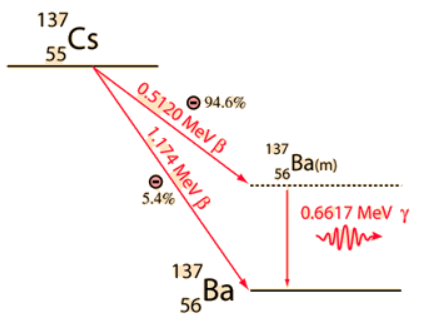
\includegraphics[width=0.5\textwidth]{bilder/decay.png}
    \caption{Zerfallsschema von Caesium 137 nach \cite{decay}.}
    \label{fig:decay}
\end{figure}
Zu erkennen ist ein anfänglicher $\beta^{-}$-Zerfall in einen Bariumzustand. 
Diese beiden Prozesse mitteln sich zu einer Halbwertszeit von $\tau_{1\text{/}2} = 30.07 \text{ Jahren}$. Der deutlich wahrscheinlichere Zerfall geht über einen angeregten Bariumzustand \ce{^{137m}_{56}Ba}. 
Dieser fällt jedoch mit einer kurzen Halbwertszeit von $\tau_{1\text{/}2} = \SI{153}{\second}$ in den stabilen Bariumzustand und gibt dabei eine charakterische Gammastrahlung ab. 
Diese Energie von $E = \SI{661.7}{\kilo\electronvolt}$ stellt den Peak des Energiespektrums von \ce{^{137}_{55}Cs} dar. Aufgrund der langen Halbwertszeit von \ce{^{137}_{55}Cs} handelt es sich um einen Dauerstrahler.
\subsection{Wechselwirkung von Gammastrahlung mit Materie}
Wenn Strahlung jeglicher Art auf ein Medium einfällt, gibt es viele wichtige Faktoren, die die Wechselwirkung mit dem Stoff bestimmen. 
Ein wichtiger Faktor stellt die Art von Strahlung dar. Oft wird hier zu erst zwischen direkt und indirekt ionisierender Strahlung unterschieden. 
Dies liegt vor allem an der Ähnlichkeit ihrer Wechselwirkungsprozesse. Neutronen zeigen eine Ahnlichkeit zu elektromagnetischer Strahlung, da sie beide keine Ladung tragen. 
Außerdem kommt es vor allem bei der Elektronenstrahlung zu weiteren Prozessen wie der Bremsstrahlung. Diese spielt bei der Photonenstrahlung nur eine sekundäre Rolle, da sie erst durch Sekundärelektronen aufkommen kann. 
In unserem Fall wird Gammastrahlung mit einem Intensitätsmaximum von $E = \SI{662}{\kilo\electronvolt}$ betrachtet. 
Die möglichen Wechselwirkungen sind hier bereits stark durch den Energiebereich und die Strahlungsart beschränkt.
Die drei wichtigsten Wechselwirkungsprozesse sind, der Photoelektrsiche Effekt, der Compton-Effekt, sowie die Paarbildung. Diese sind im Folgenden genauer beschrieben.
\subsubsection{Photoeffekt}
Der Photoeffekt beschreibt den Prozess, ein Elektron mithilfe eines Photons aus einem Atom herauszulösen, oder sein Energieniveau anzuregen. 
Er kann immer dann vorkommen, wenn die elektromagnetische Strahlung hinreichend Energie $h\nu_{\text{min}}$ besitzt, um ein Elektron aus seiner Bindung vom Atom zu lösen, oder sein Energieniveau anzuheben. 
Diese Bindungsenergie ist eine sehr spezifische Energie des jeweiligen Atoms. Die nötige Energie zum Herauslösen wird als Austrittsarbeit $W_a$ bezeichnet. 
Der Wirkungsquerschnitt gibt die Wahrscheinlichkeit für das Auftreten des betrachteten Prozesses an.
Da Gammastrahlung bereits eine im klassischen Vergleich große Energie darstellt, kann eine Näherung für große Energien des Wirkungsquerschnittes ... vorgenommen werden und es zeigt sich
\begin{equation}
\sigma^{\text{Photo}} \propto \frac{Z^{4-5}}{E} \quad | \quad \text{für hohe Energien}.
\end{equation}
Dabei entspricht $Z$ die Kernladungszahl des Absorbermaterials. 
Die Wahrscheinlichkeit für den Photoeffekt nimmt also mit steigender Photonenenergie ab, es zeigt sich allerdings, dass, in den meisten Fällen erst bei Energien einiger Megaelektronenvolt, der Compton-Effekt stark dominiert. 
Ein Abbild des Prozesses in Form eines Feynman-Diagrams ist in der Darstellung ... gezeigt.
\subsubsection{Comptoneffekt}
Die inelastische Streuung von Photon an quasi-freien Elektronen wird als Comptoneffekt bezeichnet. 
Der Energieübertrag auf das Elektron lässt sich dabei durch geometrische Betrachtungen zusammen mit Impuls- und Energieerhaltung ermitteln. Es gilt
\begin{equation}
    \increment \lambda = \frac{h}{m_e c} (1 - \text{cos}(\theta)),
\end{equation}
wobei $\theta$ den Winkel zwischen ein- und ausfallendem Photon darstellt. 
Wichtig ist, dass durch diesen Effekt neue Phänomene entstehen. Zum einen wird hier das Photon nicht vollständig aufgenommen, sondern nur um einen Energiebruchteil verringert und in eine Richtung $\theta$ gestreut. 
Dies wird sich auch durch eine erhöhte Zählrate niedirger Energien beim Einsetzen möglicher Streuobjekte in den Strahlengang zeigen. Die Winkelverteilungen und Häufigkeiten lassen sich über den Klein-Nishina-Wirkungsquerschnitt ermitteln. 
In dem Energiebereich der Gammastrahlung kommt es bereits vermehrt zum Comptoneffekt, deshalb ist dieser in dem Versuch ein auschlaggebender Prozess.
\subsection{Tomographie}
Unter der Tomographie versteht sich ein bildgebendes Verfahren, welches ein Gesamtbild aus einzelnen Schnittbildern konstruieren kann. Gemessen wird hierbei
lediglich eine Intensitätsveränderung vor- und hinter dem abzubildendem System. 
Bei dem bekannten Röntgenbild, wird die Intensitätsschwächung ins zweidimensionale projeziert, während bei der CT (Computertomographie) ein dreidimensionales Bild aus vielen Projektionen erstellt wird. 
In unserem Fall wird lediglich eine Ebene eines Materialblocks auf ihren Inhalt untersucht. Dieser lässt sich dabei aus der Messung einzelnen Intensitätsschwächungen rekonstruieren. 